\documentclass[a4paper,11pt]{article}
\usepackage{amsmath,amsthm,amsfonts,amssymb,amscd,amstext,vmargin,graphics,graphicx,tabularx,multicol} 
\usepackage[francais]{babel}
\usepackage[utf8]{inputenc}  
\usepackage[T1]{fontenc} 
\usepackage{pstricks-add,tikz,tkz-tab,variations}
\usepackage[autolanguage,np]{numprint} 
\usepackage{calc}

\setmarginsrb{1.5cm}{0.5cm}{1cm}{0.5cm}{0cm}{0cm}{0cm}{0cm} %Gauche, haut, droite, haut
\newcounter{numexo}
\newcommand{\exo}[1]{\stepcounter{numexo}\noindent{\bf Exercice~\thenumexo} : }
\reversemarginpar

\newcommand{\bmul}[1]{\begin{multicols}{#1}}
\newcommand{\emul}{\end{multicols}}

\newcounter{enumtabi}
\newcounter{enumtaba}
\newcommand{\q}{\stepcounter{enumtabi} \theenumtabi.  }
\newcommand{\qa}{\stepcounter{enumtaba} (\alph{enumtaba}) }
\newcommand{\initq}{\setcounter{enumtabi}{0}}
\newcommand{\initqa}{\setcounter{enumtaba}{0}}

\newcommand{\be}{\begin{enumerate}}
\newcommand{\ee}{\end{enumerate}}
\newcommand{\bi}{\begin{itemize}}
\newcommand{\ei}{\end{itemize}}
\newcommand{\bp}{\begin{pspicture*}}
\newcommand{\ep}{\end{pspicture*}}
\newcommand{\bt}{\begin{tabular}}
\newcommand{\et}{\end{tabular}}
\renewcommand{\tabularxcolumn}[1]{>{\centering}m{#1}} %(colonne m{} centrée, au lieu de p par défault) 
\newcommand{\tnl}{\tabularnewline}

\newcommand{\trait}{\noindent \rule{\linewidth}{0.2mm}}
\newcommand{\hs}[1]{\hspace{#1}}
\newcommand{\vs}[1]{\vspace{#1}}

\newcommand{\N}{\mathbb{N}}
\newcommand{\Z}{\mathbb{Z}}
\newcommand{\R}{\mathbb{R}}
\newcommand{\C}{\mathbb{C}}
\newcommand{\Dcal}{\mathcal{D}}
\newcommand{\Ccal}{\mathcal{C}}
\newcommand{\mc}{\mathcal}

\newcommand{\vect}[1]{\overrightarrow{#1}}
\newcommand{\ds}{\displaystyle}
\newcommand{\eq}{\quad \Leftrightarrow \quad}
\newcommand{\vecti}{\vec{\imath}}
\newcommand{\vectj}{\vec{\jmath}}
\newcommand{\Oij}{(O;\vec{\imath}, \vec{\jmath})}
\newcommand{\OIJ}{(O;I,J)}


\newcommand{\reponse}[1][1]{%
\multido{}{#1}{\makebox[\linewidth]{\rule[0pt]{0pt}{20pt}\dotfill}
}}

\newcommand{\titre}[5] 
% #1: titre #2: haut gauche #3: bas gauche #4: haut droite #5: bas droite
{
\noindent #2 \hfill #4 \\
#3 \hfill #5

\vspace{-1.6cm}

\begin{center}\rule{6cm}{0.5mm}\end{center}
\vspace{0.2cm}
\begin{center}{\large{\textbf{#1}}}\end{center}
\begin{center}\rule{6cm}{0.5mm}\end{center}
}



\begin{document}
\pagestyle{empty}
\titre{Séance d'AP 8  : Le tableur au brevet}{}{}{3ème}{}

\vspace*{0.2cm}

\setlength{\fboxrule}{2pt}
\begin{flushleft}
\framebox{\begin{minipage}{\linewidth}

\vspace*{0.2cm}

\underline{\textbf{{\large A retenir !}}}\\

\textbf{VOCABULAIRE}\\

\textbf{Cellules} \hspace*{2.25cm} Ce sont les cases.

\textbf{Plage de cellules} \hspace*{0.5cm}  C'est un ensemble de cellules. Par exemple, A1 : A10 désigne les cellules 1 à 10 de la colonne A.\\

\textbf{LES FORMULES}\\

Lorsque l'on écrit le signe « = » dans une cellule, on indique que l'on va y écrire \textbf{une formule}. \\
Ensuite, on clique sur les cellules avec lesquelles on souhaite effectuer un calcul, ou l'on écrit le nom de la cellule (par exemple, = B4 - B3), ou toute une plage de cellules (par exemple, =MIN(A1 : A10).\\

\textbf{NB} \hspace*{0.75cm} \textbf{MIN} \hspace*{0.75cm}  \textbf{MAX}   \hspace*{0.75cm}  \textbf{SOMME} \hspace*{0.75cm} \textbf{PRODUIT} \hspace*{0.75cm}  \textbf{QUOTIENT} \hspace*{0.75cm}  \textbf{MOD}\\

  \textbf{MOYENNE} \hspace*{0.75cm}  \textbf{QUARTILE} \hspace*{0.75cm}   \textbf{PGCD}  \hspace*{0.75cm} \textbf{PPCM} \hspace*{0.75cm}  \textbf{COS} \hspace*{0.75cm}  \textbf{SIN} \hspace*{0.75cm} \textbf{TAN}       
 


\end{minipage}}
\end{flushleft}

\vspace*{0.7cm}


\exo

Le tableau fournit le nombre d'exploitations agricoles en France, en fonction de leur surface pour les années 2000 et 2010.\\

\includegraphics[scale=1]{tableur1.eps} \\

\q  Quelles sont les catégories d'exploitations qui ont vu leur nombre augmenter entre 2000 et 2010 ?\\

\q Quelle formule doit-on saisir dans la cellule B8 pour obtenir le nombre total d'exploitations agricoles en 2 000 ?\\

\q Si on étire cette formule, quel résultat s'affiche dans la cellule C8 ?\\

\q Peut-on dire qu'entre 2000 et 2010 le nombre d'exploitations de plus de 200 $ha$ a augmenté de 40 $\%$ ? Justifier\\

\newpage

\exo

On considère 2 fonctions $f$ et $g$ telles que  
\begin{center}
$ f(x) = -8x$ et $g(x)=-6x+4$
\end{center}
On utilise un tableur pour calculer des images par $f$ et $g$.\\

\includegraphics[scale=1]{tableur2.eps} \\

\initq \q Quelle formule peut-on saisir dans la cellule B2 avant de la recopier vers la droite ?\\

\q Le contenu de la cellule E1 a été effacé. Quel est ce contenu ?\\

\q On fabrique une nouvelle fonction $h$ telle que $h(x)=f(x) \times g(x)$. La fonction $h$ est-elle une fonction affine ?\\



\exo

Une station de ski a relevé le nombre de forfaits « journée » vendus lors de la saison écoulée (de décembre à avril).\\
Les résultats sont donnés ci-dessous dans la feuille de calcul d'un tableur.\\

\includegraphics[scale=1]{tableur3.eps} \\

\noindent \initq \q \qa Quel est le mois durant lequel la station a vendu le plus de forfaits « journée » ?\\
 \qa Ninon dit que la station vend plus du tiers des forfaits durant le mois de février. A-t-elle raison? Justifier.\\
 
\q Quelle formule doit-on saisir dans la cellule G2 pour obtenir le total des forfaits « journée » vendus durant la saison considérée ?\\

\q Calculer le nombre moyen de forfaits « journée » vendus par la station en un mois. On arrondira le résultat à l'unité.\\

\vspace*{0.25cm}

\exo 

Le tableau ci-dessous a été réalisé à l'aide d'un tableur.\\
Il indique le nombre d'abonnements Internet à haut débit et à très haut débit entre 2014 et 2016, sur réseau fixe, en France. \textit{(Sources : Arcep et Statistica)}.\\

\includegraphics[scale=1]{tableur5.eps} \\

\initq \q Combien d'abonnements Internet à très haut débit, en millions, ont été comptabilisés pour l'année 2016 ?\\

\q Vérifier qu'en 2016, il y avait 817 000 abonnements Internet à haut débit et à très haut débit de plus qu'en 2015.\\

\q Quelle formule a-t-on pu saisir dans la cellule B4 avant de la recopier vers la droite, jusqu'à la cellule D4 ?\\

\q En 2015, seulement 5,6 $\%$ des abonnements Internet à très haut débit utilisaient la fibre optique. Quel nombre d'abonnements Internet à très haut débit cela représentait-il ?\\







\end{document}
